\section{Memory \& Paging}

\begin{frame}{Overview: Memory \& Paging}
	\begin{itemize}
		\setlength\itemsep{1em}
		\item Paging: Abstract physical memory from virtual address spaces
		\item New pages can be mapped in/out dynamically
		\item Use of different address spaces for process separation
		\item Kernel is mapped at 3 GiB $\rightarrow$ Higher-Half-Kernel (always visible)
		\item Adresses below 3 GiB are used for user space memory
	\end{itemize}	
\end{frame}

\begin{frame}{Paging: The boot process}
	\begin{itemize}
		\item How to allocate memory when no memory manager is available?
		\item How to map the Kernel-code at 3 GiB without losing the EIP?
		\item Solution: Activate paging in several steps
	\end{itemize}
	\pause
	\begin{figure}
		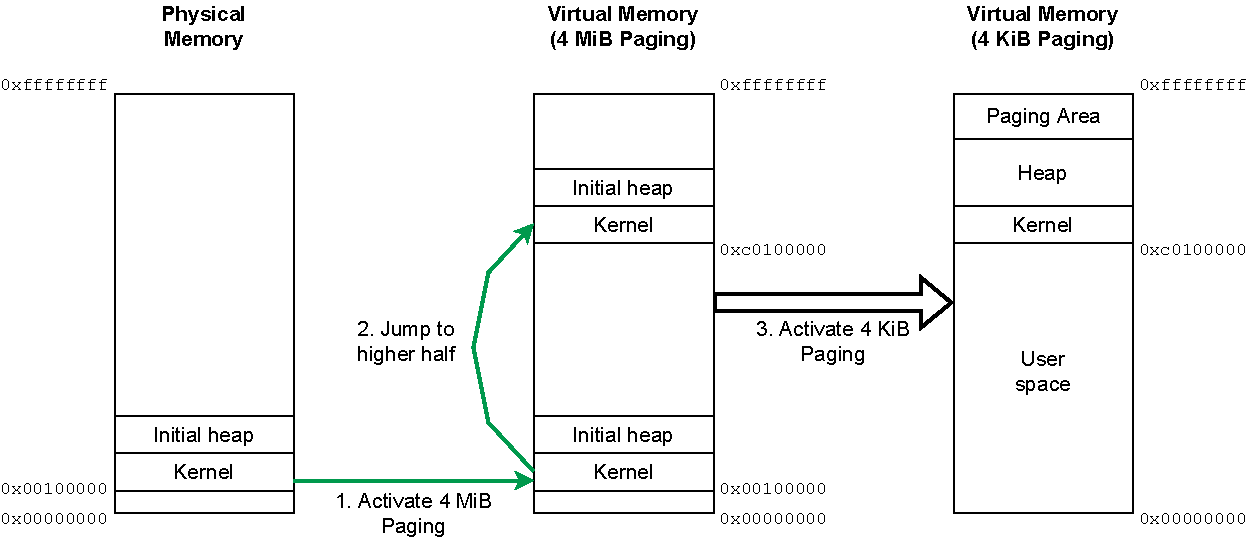
\includegraphics[width=0.9\textwidth]{img/paging}
	\end{figure}
\end{frame}

\begin{frame}{Allocating heap memory}
	\begin{enumerate}
		\setlength\itemsep{1em}
		\item Invoke Free list manager to find free memory block in heap
		\item Slice free block (with respect to alignment)
		\item Return pointer to found block
		\item If the block was not previously mapped, the first access will generate a pagefault
		\item Fault handler is invoked during interrupt handling
		\item Search unused pageframe and map it to the virtual fault address
		\item Return to program
	\end{enumerate}
\end{frame}